\chapter{Система квантового распределения ключа на поднесущих гармониках с применением двух независимых источников когерентного излучения на непрерывных переменных}\label{ch:ch3}
Первые системы квантового распределения ключа на непрерывных переменных основывались на генерации и локального осциллятора, и квантовых состояний, одним лазером. Это позволяло избегать проблем с рассогласованием фаз ЛО и квантовых состояний. Однако, это несло и существенные недостатки. Была необходима система мультиплексирования на стороне передатчика и демультиплексирования на стороне приемника для того, чтобы была возможность передавать локальный осциллятор в одном же волокне с квантовыми состояниями без нежелательной интерференции ЛО с ними. Другим недостатком являлась ограниченная мощность передаваемого локального осциллятора. Это связано с несколькими причинами. Первая причина - при передаче по ВОЛС локальный осциллятор затухает как и все сигналы, проходящие по волокну, что ограничивает его мощность на этапе интерференции в приемном модуле. Вторая причина ограничения мощности локального осциллятора - нелинейные эффекты, возникающие во время прохода мощного сигнала по волоконно-оптическому тракту, связанный с рассеянием Релея и прочими. Соответственно, передача мощного ЛО может перекрыть все преищмуества его мощности дополнительными шумамами. И самая главная проблема - это возможные атаки на ЛО от злоумышленника. Итогом всех этих проблем стало использование "локального" локального осциллятора на стороне приемника, сгенерированного отдельным независимым лазером.
\section{Метод гетеродинного детектирования сигналов для системы квантового распределения ключа на боковых частотах}\label{sec:ch3/sec1} 
В данной главе предлагается использование гетеродинного метода детектирования сигнала с применением двух независимых источников когерентного излучения на непрерывных переменных. Данный способ обладает следующими достоинствами
\begin{enumerate}
    \item Использование источника ЛО на стороне приемника решает проблемы передачи ЛО в канале, связанные с шумом и недостаточной мощностью
    \item Оптическая схема с ЛО на стороне приемника защищает этот источник от атак злоумышленника, что существенно повышает устойчивость данной системы к воздействию злоумышленника
    \item При гетеродинном приеме сигнала, информация о принятом сигнале переносится в полосу радиочастот на промежуточную частоту, что позволяет анализировать и усиливать гармоническое колебание, что существенно расширяет возможность по применяемым видам модуляции
    \item Применение гетеродинного метода детектирования сигналов также позволяет разделять частотно-мультиплексированные сигналы на одну несущую оптическую частоту для повышения скорости выработки секретного ключа или повышения секретности за счет случайного выбора рабочей частоты.
\end{enumerate}
Современные работы по созданию систем КРК на непрерывных переменных переходят к использованию ЛО, сгенерированного на стороне приемника. В данной работе рассматривается применение двух независимых источников излучения для системы квантового распределения ключа на поднесущих гармониках и с частотным мультиплексированнием на одной несущей частоте.
\section{Протокол квантового распределения ключа на поднесущих гармониках с гетеродинном методом детектирования сигналов}\label{sec:ch3/sect2}
Протокол работает следующим образом:
\begin{enumerate}
    \item Алиса готовит квантовые состояния, кодируя информацию в фазовый свиг излучения на боковых частотах ослабленного лазерного излучения, и передает их.
    \item Боб измеряет пришедшие квантовые состояния с помощью гетеродинного детектирования.
    \item Выходной сигнал балансного детектора оцифровывается и обрабатывается с помощью алгоритма Быстрого Преобразования Фурье.
    \item Измеряется частота и фаза нужной гармоники из полученного мгновенного спектра.
    \item Оценивается соотношение сигнал/шум.
    \item Проводится процедура исправления ошибок с помощью соответствующих кодов.
\end{enumerate}
\section{Оптическая схема системы квантового распределения ключа на боковых частотах с применением гетеродинного детектирования }\label{sec:ch3/sect5}
Данная схема устроена следующим образом. Лазер на стороне передатчика генерирует непрерывное лазерное излучение. Это излучение проходит по оптическому волокну с сохранением поляризации  и попадает на фазовый модулятор. На фазовый модулятор попадает сигнал от генератора сигналов свободной формы. Этот генератор подготавливает модулирующий сигнал. В нем содержаться фазовые сдвиги, которые соответствуют кодировке QPSK  с фазами 45, 135, 215 и 305 градусов. Этот сигнал модулирует оптическое излучение и на выходе получаются дополнительные поднесущие гармоники сигнала в выходном спектре фазового модулятора. После этого сигнал попадает на волоконно-оптический перестраиваемый аттенюатор для снижения уровня мощности на поднесущих гармониках до однофотонного уровня.
После этого сигнал проходит квантовый канал и попадает на схему контроля поляризации, которая рассматривается в секции \ref{sec:ch3/sect4}. После прохождения этой схемы, сигнал попадает на светоделитель с 2 входами и 2 выходами с коэффициентом деления 50:50, на входы которого попадает и сигнал локального осциллятора. В результате происходит интерференция этих сигналов. Но частоты ЛО и информационного сигнала отличаются так, что частота ЛО больше частоты лазера передатчика. В итоге этот результат интерференции регистрируется балансным детектором. Разностные частоты от всех сигналов, которые проинтерферировали, находятся в полосе пропускания балансного детектора благодаря подбору частот. При необходимости частота лазера ЛО может быть подстроена для переноса спектра сигнала вверх или вниз по частоте. По итогу на выходе БД формируется несколько гармонических колебаний. Для анализа необходимо отфильровать синусоидальное колебание на частоте модуляции, так как оно несет информацию о фазе, закодированной передатчиком. После этого его можно обрабатывать уже методами цифровой обработки сигналов (ЦОС). Для компенсации же фазовых искажений можно обрабатывать промежуточную частоту между лазерами передатчика и  приемника. Ее фазовые колебания будут содержать фазовый шум и передатчика с квантовым каналом, и фазовый шум ЛО. Это измеренное значение необходимо учитывать на этапе постобработки. 
Оптическая схема гетеродинного метода детектирования для системы КРК приведена на рисунке \ref*{fig:het true ch3} 
\begin{figure}
    \centering
    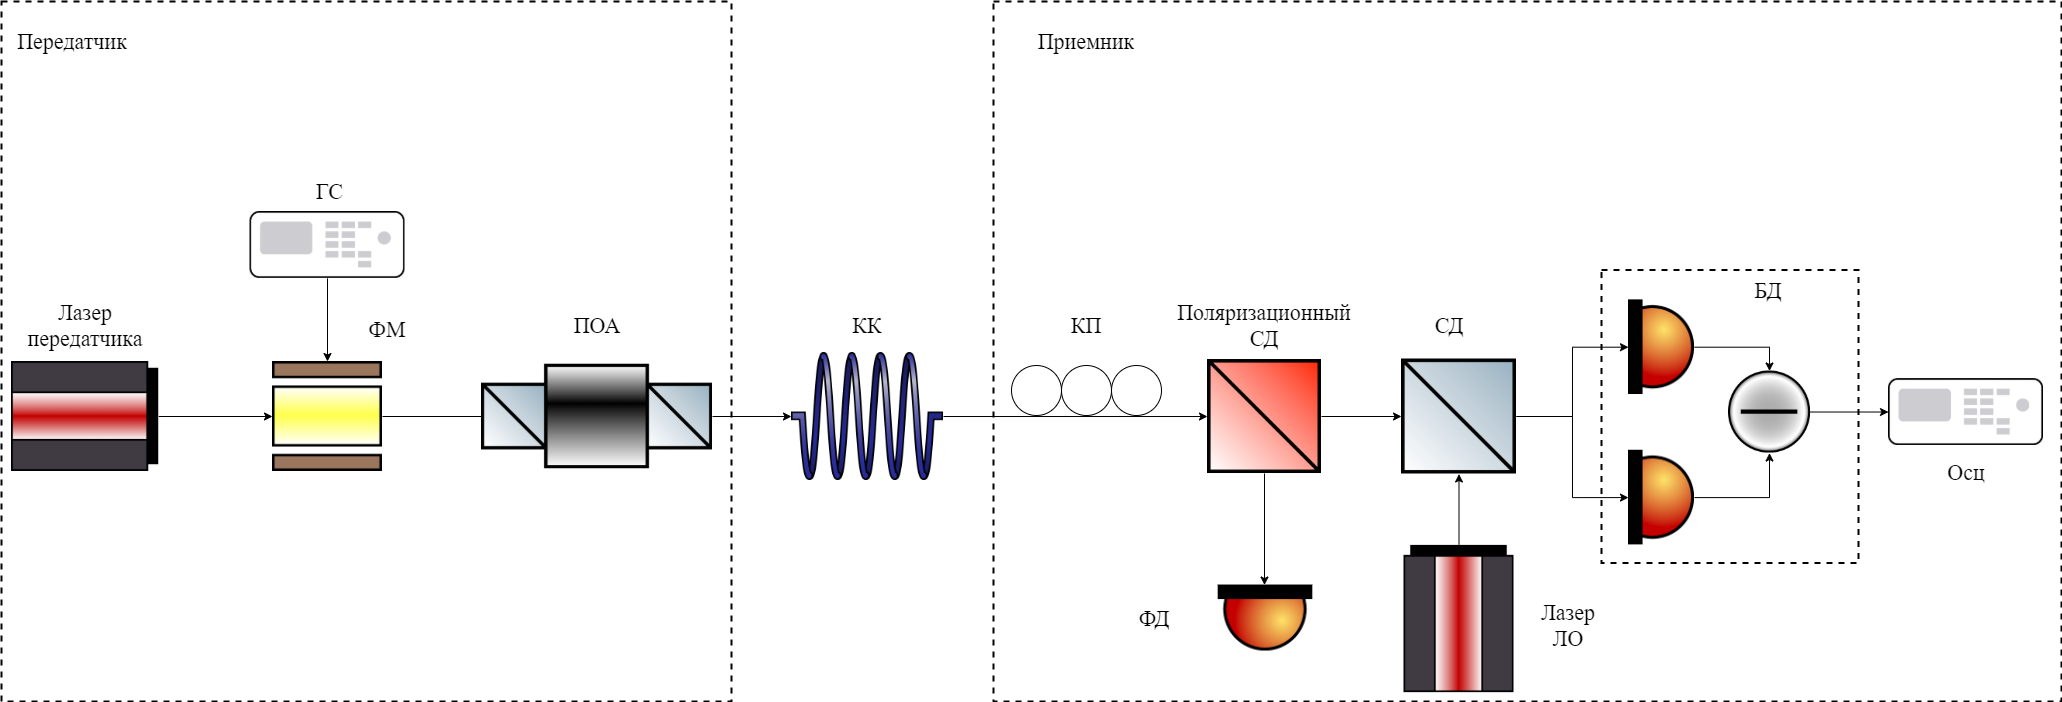
\includegraphics[width = \textwidth]{images/Гетеродин схема новая2 .png}
    \caption{Схема эксперимента по реализации гетеродинного метода приема сигналов для КРК, где ГС - генератор сигналов, ФМ - фазовый модулятор, ПОА - перестраиваемый оптический аттенюатор, КК - квантовый канал, КП - контроллер поляризации, СД - светоделитель, ФД - фотодиод, ЛО - локальный осциллятор, БД - балансный детектор, ОСЦ - осциллограф}
    \label{fig:het true ch3}
\end{figure}
\section{Математическая модель системы квантового распределения ключа на боковых частотах с применением гетеродинного детектирования}\label{sec:ch3/sect3}
Излучение лазера может быть представлено следующим образом:
\begin{align}
F(t) = A_0 * \sin(\omega_0 t + \phi_0),
\end{align}
где $A_0$ -- амплитуда сигнала, $\omega_0$ -- частота лазерного излучения, $\phi_0$ -- начальная фаза излучения.
Модулирующий сигнал:
\begin{align}
S(t) = (1+ m\sin(\Omega t  + \phi (t))),
\end{align} 
где $m$ -- индекс модуляции, $\Omega$ -- частота модуляции, $\phi (t)$ -- вносимая модуляция.

Лазерное излучение после модуляции выглядит следующим образом:
\begin{align}
\label{eq:laser}
F_s(t) &= F(t) * S(t) = A_0 * \sin(\omega_0 t + \phi_0) + \frac{A_0 * m}{2} * (\cos((\omega_0 + \Omega)t + (\phi_0 + \phi (t))) - \notag \\
&- \frac{A_0 * m}{2} * (\cos((\omega_0 - \Omega)t + (\phi_0 - \phi (t))),
\end{align}

Результат квадратичного детектирования сигнала, полученного в выражении~\eqref{eq:laser} будет выглядеть следующим образом:
\begin{align}
F_d(t) &= F(t)^2 * S(t)^2 = (A_0 * \sin (\omega_0 t + \phi_0))^2 * (1 + m*\sin (\Omega t + \phi_0 + \phi (t))^2=\notag \\
&= \frac{1}{8}\bigg \{4A_0^2 + 2A_0^2 *m^2 - 4A_0^2\cos(2\omega t + 2\phi_0) - 2A_0^2*m^2\cos(2\omega t + 2\phi_0) - \notag \\ & - 2A_0^2*m^2\cos(2\Omega t + 2\phi(t))  + A_0^2*m^2\cos(2\omega t - 2\Omega t + 2\phi_0 - 2\phi(t)) + \notag \\ & + A_0^2*m^2\cos(2\omega t + 2\Omega t + 2\phi_0 + 2\phi(t)) + 8A_0^2m\sin(\Omega t + 2\phi(t)) -\notag \\ & + 4A_0^2m\sin(2\omega t - \Omega t +2\phi_0 - \phi(t)) - 4A_0^2m\sin(2\omega t + \Omega t + 2\phi_0 + \phi(t))   \bigg\},
\end{align}
В результате ток, протекающий через фотодиод, будет определяться выражением:
\begin{align}
   I &= R(\lambda)G C F_d,
\end{align} 
где $R(\lambda)$ -- спектральная чувствительность фотодиода, $G$ -- электрическое усиление балансного детектора, $C$ -- отношение апертуры волокна к размеру чувствительной площадки фотодетектора. 

В случае проводимого эксперимента единственная гармоника, которая лежит в полосе пропускания балансного детектора -- это  $A_0^2m*\sin(\Omega t   + \phi (t))$.
Остальные же гармоники не попадают в полосу пропускания и будут проявляться в виде постоянной составляющей, которая отфильтровывается перед первым усилителем. 

\section{Алгоритм подстройки поляризационных искажений для системы квантового распределения ключа на боковых частотах с применением гетеродинного детектирования}\label{sec:ch3/sect4}
Существенной проблемой для интерференции сигналов является их поляризация. Как известно, сигналы в ортогональный поляризациях не взаимодействуют. Что существенно снижает эффективность передачи данных в системах КРК на непрерывных переменных. В рамках данного раздела предалаегся реализация алгоритма подстройки поляризации пришедшего сигнала.
При использовании связки поляризационного светоделителя и контроллера поляризации можно подстраивать поляризацию за счет анализа спектрального состава принятного сигнала с помощью быстрого преобразования Фурье. В случае неправильной поляризации, на выходе поляризационного светоделителя сигнал разделяется на две поляризации по осям: быструю и медленную. В итоге получается так, что на балансный детектор приходят два сигнала, а не один. Это приводит к тому, что в спектре полученного сигнала появляется не только гармоника на частоте модуляции, но и ее удвоение. Что можно отслеживать и использовать контроллер поляризации для контроля входной поляризации. На рисунке \ref{fig:ruin pol}
\begin{figure}
    \centering
    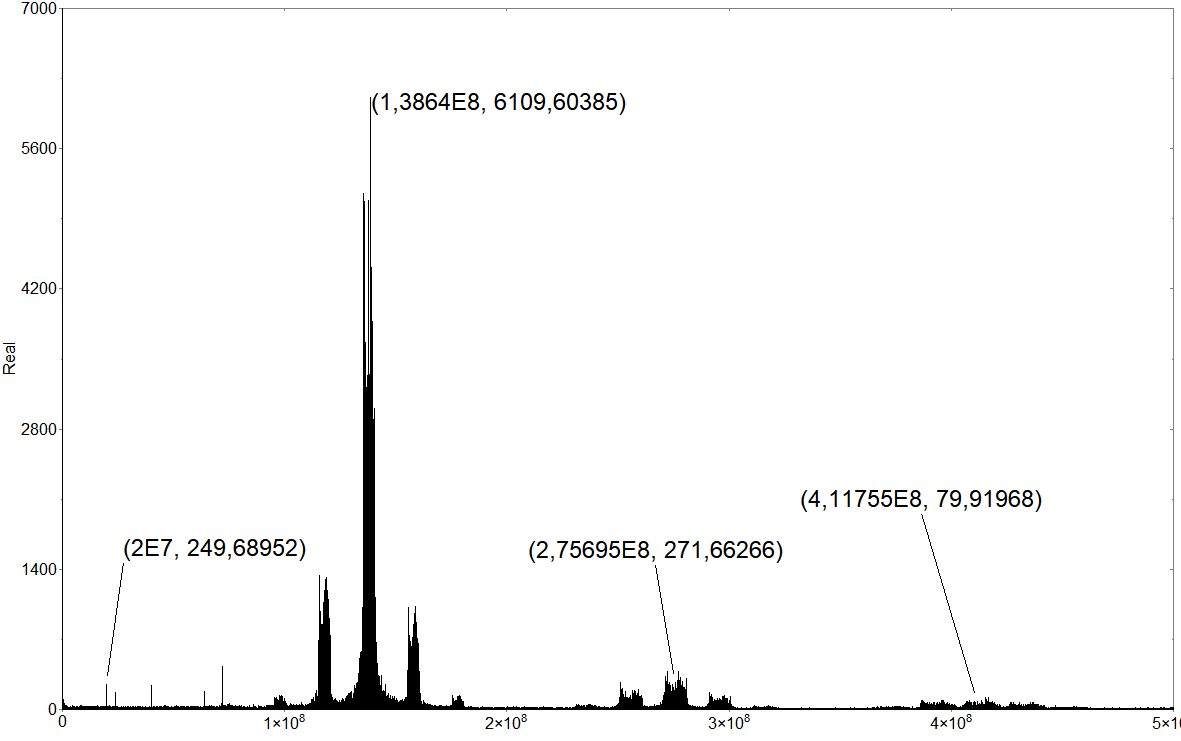
\includegraphics[width = \textwidth]{images/Spectrum of ruined polarization.png}
    \caption{Спектр выходного сигнала с неправильной поляризацией }
    \label{fig:ruin pol}
\end{figure}
В спектре этого сигнала наблюдается гармоники на частоте 20 МГц, что соответствует частоте модулирующего излучения и 40 МГц, что является удвоенной частотой модуляции. На основе этой информации система обратной связи должна дать команду на контроллер поляризации для ее контроля. В результате действий КП должен приветси сигнал к виду, отображенному на рисунке \ref{fig:norm pol}
\begin{figure}
    \centering
    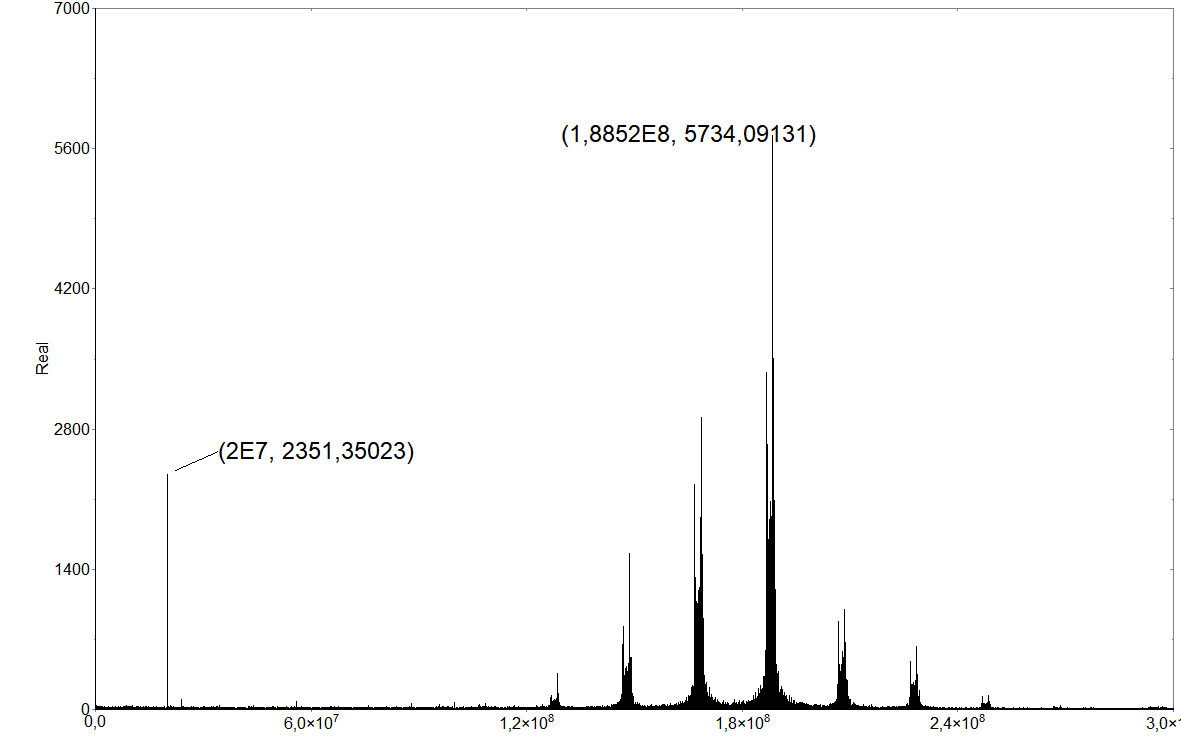
\includegraphics[width = \textwidth]{images/normal polarization.png}
    \caption{Спектр выходного сигнала с балансного детектора с правильной поляризацией}
    \label{fig:norm pol}
\end{figure}
На графике \ref{fig:norm pol} видно, что присутствует только спектральная линия от частоты модуляции и по амплитуде она существенно больше, чем на графике \ref{fig:ruin pol}. 
В общем виде алгоритм можно записать следующим образом
\begin{enumerate}
    \item Применение БПФ к принятому сигналу
    \item Анализ спектрального состава сигнала
    \item Поворот поляризации сигнала до уничтожения гармоники на удвоенной частоте модуляции
    \item Дальнейший поворот поляризации сигнала до максимума гармоники на частоте модуляции
\end{enumerate}
\section{Математическая модель гетеродинного детектирования с двумя независимыми источниками излучения}\label{sec:ch3/sect6}
\section{Описание экспериментальной установки}\label{sec:ch3/sect7}
Для реализации системы квантового распределения ключей на поднесущих гармониках с применением двух независимых источников излучения на непрерывных переменных была собрана экспериментальная схема изображенная на рисунке \ref*{fig:het true ch3}
Данная схема работает следующим образом. Лазерное излучение, сгенерированное лазером NeoPhotonics $\mu$ITLa с шириной линии менее 100 кГц и выходной мощностью 1 мВт и длиной волны 1550.0026 нм. В качестве лазера локального осциллятора использовался лазер Hewlett & Packard 8168C с излучением на длине волны 1550.0018 нм и выходной мощностью 1 мВт. В качестве фазового модулятора использовался фазовый модулятор производства EOSpace с полосой пропускания 40 ГГц и вносимыми потерями 4 дБ.
В качестве балансного детектора использовался детектор фирмы General Photonics BDP-003 с чувствительностью 0.8 А/Вт на длине волны 1550 нм, полосой пропускания 200 МГц и коэффициентом усиления ${10^5}$.
Для измерений и выполнения Быстрого Преобразования Фурье использовался осциллограф Rohde & Schwarz RTM 3000  с полосой пропускания 1 ГГц и количеством выбором 5 ГВ/с.
На электрический же вход фазового модулятора подается гармонический синусоидальный  сигнал с частотой 20 МГц и амплитудой 1 В и дополнительным смещением в 0.8 В. В результате взаимодействия лазерного излучения и электрического сигнала на фазовом модуляторе в спектре излучения образуются 2 дополнительные гармоники - боковые частоты.
Полученный сигнал попадает на переменный оптический аттенюатор, который вносит затухание таким образом, чтобы на боковых частотах был уровень сигнала, мощность которого в среднем меньше мощности одного фотона.
После этого полученный сигнал передается по одномодовому оптическому волокну на сторону приемника. Попав на сторону приемника, сигнал попадает на блок контроля поляризации, о принципе работы которого будет рассказано позже. Прошедший сигнал попадает на один из входов светоделителя с 2 входами и 2 выходами и коэффициентом деления 50:50.
На другой же вход светоделителя попадает излучение лазера - локального осциллятора (ЛО). В результате на светоделителе квантовые состояния от Алисы интерферируют с локальным осциллятором. За счет этой интерференции с мощным ЛО, квантовые состояния усиливаются и регистрируются балансным детектором, который основан на двух классических фотодиодах.

\section{Описание полученных результатов}\label{sec:ch3/sect8}
При интерференции локального осциллятора и квантовых состояний, посланных Алисой, на светоделителе на стороне Боба, формируются комбинационные частоты от всех спектральных составляющих. Их модели описаны в разделе \ref*{sec:ch3/sect6}.
В полученной модели интерес представляют только разностные частоты по причине того, что только они попадают в полосу пропускания балансного детектора.
На выходе балансного детектора формируется гармонический сигнал состоящий из двух огибающих и несущей. Форма этого сигнала изображена на рисунке \ref*{fig: het true time}
\begin{figure}
    \centering
    \includegraphics*{толстые линии и исправлены названия сигнал после детектирования.png}
    \caption*{Выходной сигнал с балансного детектора во временной области}
    \label{fig: het true time}
\end{figure}
Информацию несут только огибающие данного сигнала. Для их анализа их предварительно необходимо отфильтровать. Это можно сделать как программными методами, так и с помощью физических фильтров, установленных после балансного детектора.
В рамках данной работы предлагается программно фильтровать огибающую, которая соответствует частоте $(\omega_{LO} -(\omega_{car} - \Omega_{mod})$, так как она попадает в полосу пропускания балансного детектора. 

В результате работы данной системы на выходе балансного детектора формируются сигналы на промежуточных частотах, которые соответствуют разности частот локального осциллятора и частот сигналов, пришедших от Алисы. Спектр сигнала изображен на рисунке \ref*{label}
\section{Определение фазового шума}\label{sec:ch3/sect9}

\section{Выводы по главе}\label{sec:ch3/sect10}